\section{Simple crane model}\label{sec:craneSimulon}
In this section, we explore the simulation of a simple crane system, examining its motion and various aspects of its configuration, as illustrated in Figure~\ref{fig:ex_reeving_system}. Utilizing the Arbitrary Lagrangian-Eulerian Modal approach, we analyze the crane's slewing and winding motions and their respective velocity profiles, while also discussing the kinematic description of the wire-rope elements.

\subsection{Description of the simple crane model}
The example simulates the motion of a simple crane. The configuration of the system is shown in Figure~\ref{fig:ex_reeving_system}. The parameters of the system are given in Table~\ref{tab:reeving_system_parameters}. As sketched in Figure~\ref{fig:ex_reeving_system}, the system subjected to two imposed motions: rotation of the crane around the vertical $Z$ axis, or \textit{slewing motion}, and rotation of the drive reel to lift the payload, or \textit{winding motion}. The velocity profiles of the winding motion and slewing motion start at zero and smoothly reach a constant value following the laws: 

\begin{equation}
V = \left\{ {\begin{array}{*{20}{c}}
\frac{1}{2}V_c(1-\text{cos}(\frac{\pi t}{t_c}))&t < t_c\\
V_c&t \ge t_c
\end{array}} \right.
 \label{eq:rotation_angle}
\end{equation}


\begin{equation}
\Omega = \left\{ {\begin{array}{*{20}{c}}
\frac{1}{2}\Omega_c(1-\text{cos}(\frac{\pi t}{t_c}))&t < t_c\\
\Omega_c&t \ge t_c
\end{array}} \right.
 \label{eq:rotation_angle}
\end{equation}

\setlength{\parindent}{0cm}
where the assumed constant velocity values are $V_c = 1\, {\rm{m}}/{{\rm{s}}}$, and $\Omega_c = 0.3\, {\rm{rad}}/{{\rm{s}}}$, and the acceleration period is $t_c = 0.2 \,s$ for both motions.

\begin{table}[tbph]
    \caption{Reeving system parameters} \label{tab:reeving_system_parameters}
    \centering
    %\begin{tabular}{@{}lrlp{0.4\textwidth}@{}} \toprule
    \begin{tabular}{c|c|c|c} \hline
        Parameter & Value & Units & Description \\ \hline
        $d$ & 
            3 & \si{\meter} & 
            Distance between drive reel and deviation pulley \\
        $l_0$ & 
            8 & \si{\meter} & 
            Undeformed length of the vertical rope span at $t = 0$ \\
        $b$ & 
            0.3 & \si{\meter} & 
            Half side of cubic payload \\
        $R$ & 
            \num{0.1} & \si{\meter} & 
            Radius of the drive reel and deviation pulley \\
        $\rho A$ & 
            \num{0.6205} & \si{\kilo\gram\per\meter} & 
            Wire ropes linear density \\
        $EA$ & 
            \num{16.5} & \si{\mega\newton} & 
            Axial stiffness \\
        $EI$ & 
            \num{30.9} & \si{\newton\meter\squared} & 
            Bending stiffness \\
        $M$ & 
            1000 & \si{\kilo\gram} & 
            Mass of the payload \\ \hline
        %\bottomrule
    \end{tabular}
\end{table}

The simulation procedure is the Arbitrary Lagrangian-Eulerian Modal approach described in ~\cite{Escalona2022, Escalona2017}. All details about the formulation can be found in the reference papers. The model includes 1 rigid body which is the payload, and 2 wire-rope elements. The total set of coordinates is given by:

\begin{equation}
    {{\bf{p}}} = {\left[ {\begin{array}{*{20}{c}}{{\bf{q}}^{2}}^T & {{\bf{q}}^{a}}^T & {{\bf{q}}^{b}}^T \end{array}} \right]^T}
    \label{CoordinateS2}
\end{equation}

\setlength{\parindent}{0cm}
where ${{\bf{q}}^{2}}$ is the set of coordinates of rigid body 2. These are 3 transnational coordinates and 4 Euler parameters:

\begin{equation}
    {{\textbf{q}}}^{2} = {\left[ {\begin{array}{*{20}{c}}{\textbf{r}^{2}}^T&{\boldsymbol{\theta}^{2}}^T \end{array}} \right]^T}
\end{equation}

\begin{equation}
  {\textbf{r}}^{2} = {\left[ {\begin{array}{*{20}{c}}{{{{r}}_x^{2}}^T}&{{{{r}}_y^{2}}^T}&
  {{{{r}}_z^{2}}^T} \end{array}} \right]^T},     \boldsymbol{\theta}^{2} = {\left[ {\begin{array}{*{20}{c}}{{\theta_{0}^{2}}}&{{\theta_{1}^{2}}}&{{\theta_{2}^{2}}}&{{\theta_{3}^{2}}}\end{array}} \right]^T}  
\end{equation}

\begin{figure}
    \centering
    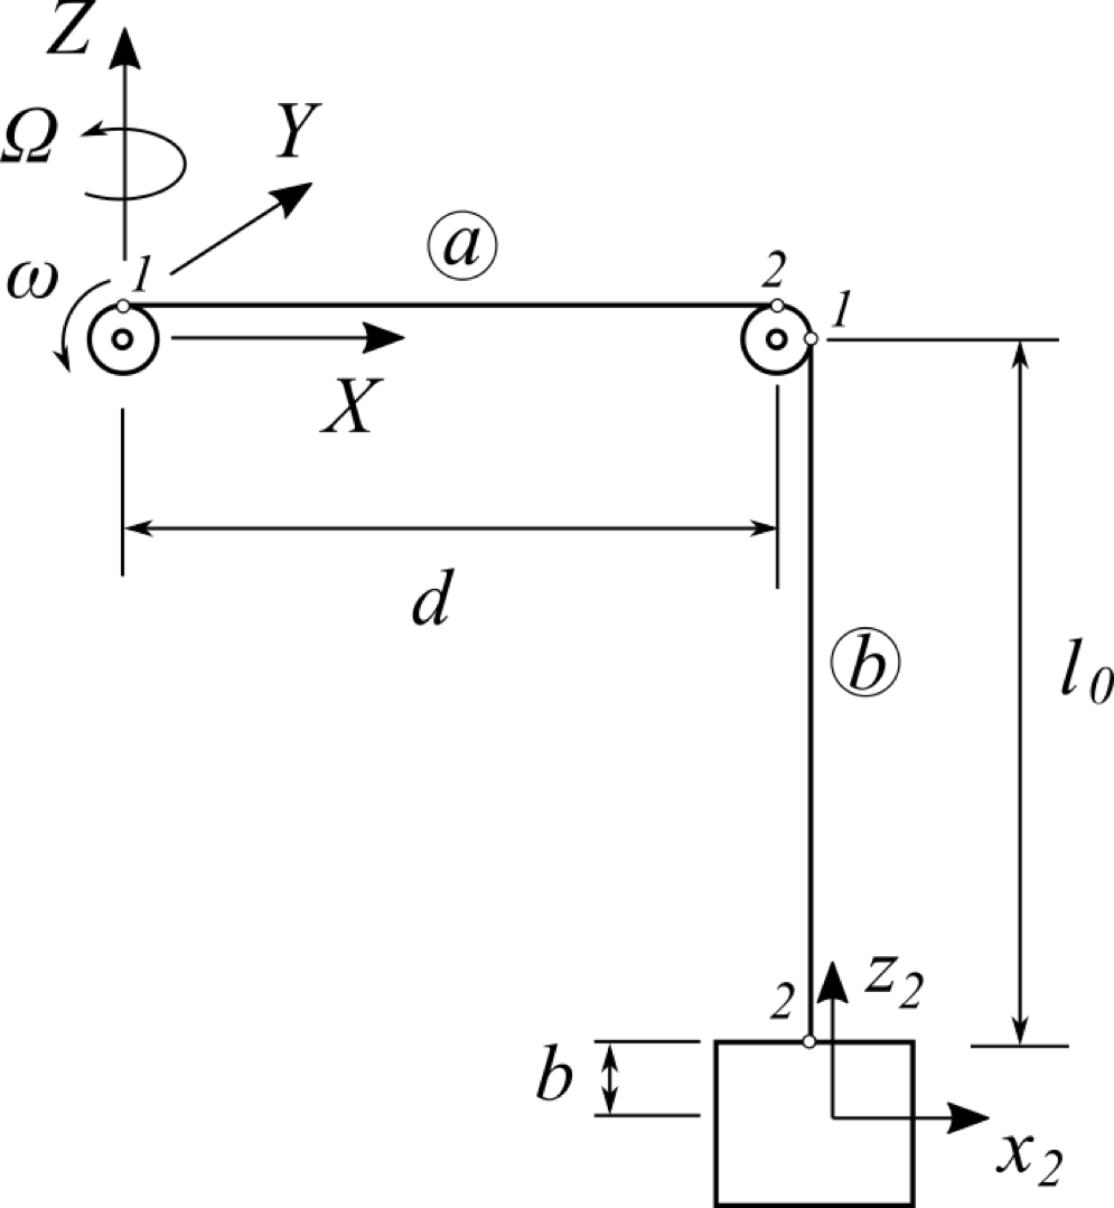
\includegraphics[width=0.4\textwidth]{Figures/simpleCrane.png}
    \caption{ALEM model of the reeving system of a simple crane}
    \label{fig:ex_reeving_system}
\end{figure}

Each ALEM wire-rope element $a$ and $b$ is kinematically described with a set of 6 absolute nodal coordinates $\textbf{q}_a$, 2 arc-length material coordinates $\textbf{q}_s$, and a maximum of 3 modal coordinates in each of the 3 local directions included in $\textbf{q}_m$. For example, for the wire-rope $a$, these coordinates are given by:

\begin{equation}
  {\textbf{q}}_a^{a} = {\left[ {\begin{array}{*{20}{c}}{{{\bf{q}}_a^{a}}^T}&{{{\bf{q}}_s^{a}}^T} & {{{\bf{q}}_m^{a}}^T} \end{array}} \right]^T}
\end{equation}

\begin{equation}
  {\textbf{q}}_a^{a} = {\left[ {\begin{array}{*{20}{c}}{{{\bf{r}}_1^{a}}^T}&{{{\bf{r}}_2^{a}}^T} \end{array}} \right]^T},     {\bf{q}}_s^{a} = {\left[ {\begin{array}{*{20}{c}}{{s_1^a}}&{{s_2^a}}\end{array}} \right]^T}  
\end{equation}

\begin{equation}
    {\textbf{q}}_m^{a} = \left[ {\begin{array}{*{20}{c}}{{q_{x,1}^a}}&{{q_{x,2}^a}} &{{q_{x,3}^a}}&{{q_{y,1}^a}}&{{q_{y,2}^a}}& {{q_{y,3}^a}}&{{q_{z,1}^a}}&{{q_{z,2}^a}}& {{q_{z,3}^a}}\end{array}} \right]^T 
\end{equation}

In this example, no modal coordinates are considered for the rope element $a$. For the rope element $b$, 3 axial-modal coordinates in the longitudinal direction $X_b$, $q_{mXi}^b,\, i = 1,2,3$, 1 transverse-modal coordinate in the local direction $Y_b$, $q_{mY1}^b$, and 1 transverse-modal coordinate in the local direction $Z_b$, $q_{mZ1}^b$, are used in the model. Therefore, the set of total coordinates $\textbf{p}$ is subjected to linear and nonlinear constraints. The linear constraints are expressed as:

\begin{equation} \label{Clin_Elev}
{{\bf{C}}_{lin}}\left( {{\bf{p}},t} \right) = \left[ {\begin{array}{*{20}{c}}
{{\bf{r}}_1^a - \left[ {\begin{array}{*{20}{c}}
0&0&R
\end{array}} \right]{}^T}\\
{{\bf{r}}_2^a - \left[ {\begin{array}{*{20}{c}}
{d\cos \alpha (t)}&{d\sin \alpha (t)}&R
\end{array}} \right]{}^T}\\
{{\bf{r}}_1^b - \left[ {\begin{array}{*{20}{c}}
{\left( {d + R} \right)\cos \alpha (t)}&{\left( {d + R} \right)\sin \alpha (t)}&0
\end{array}} \right]{}^T}\\
{{\bf{r}}_2^b - \left( {{{\bf{r}}^2} + {{\bf{A}}^2}\left[ {\begin{array}{*{20}{c}}
0&0&b
\end{array}} \right]{}^T} \right){}^T}\\
{s_1^a - \int {Vdt} }\\
{s_2^a - s_1^b}\\
{s_2^b - \left( {d + {l_0}} \right)}\\
{{\bf{q}}_m^a}\\
{q_{mY2}^b}\\
{q_{mY3}^b}\\
{q_{mZ2}^b}\\
{q_{mZ3}^b}
\end{array}} \right] = {\bf{0}}
\end{equation}

\setlength{\parindent}{0cm}
This is a set of 28 equations, $m_l = 28$.\\     

Nonlinear constraints are due to the force balance of the wire rope elements at the deviation sheave and to the unity of the quaternions used to describe the rotation of the payload, as follows: 

\begin{equation} 
{{\bf{C}}_{nonlin}}\left( {\bf{p}} \right) = \left[ {\begin{array}{*{20}{c}}
{F_{ax2}^a\left( {{{\bf{q}}^a}} \right) - F_{ax1}^b\left( {{{\bf{q}}^b}} \right)}\\
{{{\left( {\theta _0^2} \right)}^2} + {{\left( {\theta _1^2} \right)}^2} + {{\left( {\theta _2^2} \right)}^2} + {{\left( {\theta _3^2} \right)}^2} - 1}
\end{array}} \right] = {\bf{0}}
\label{WRnl}
\end{equation}

\setlength{\parindent}{0cm}
This is a set of 2 equations, $m_{nl} = 2$.\\

The number of generalized coordinates $\textbf{q}$ of the system , $n$, equals the number of coordinates in $\textbf{p}$, $n_p$, minus the number of linear constraints: $n = {n_p} - {m_l} = 41 - 28 = 13$.
The array $\textbf{q}$ is given by:

\begin{equation} \label{setq_Elev}
{\bf{q}} = {\left[ {\begin{array}{*{20}{c}}
{r_x^2}&{r_y^2}&{r_z^2}&{\theta _0^2}&{\theta _1^2}&{\theta _2^2}&{\theta _3^2}&{s_2^a}&{q_{mX1}^b}&{q_{mX2}^b}&{q_{mX3}^a}&{q_{mY1}^b}&{q_{mZ1}^b}
\end{array}} \right]^T}
\end{equation}

The generalized coordinates of the system $\textbf{q}$ is partitioned into independent coordinates, $\textbf{q}_{ind}$, and dependent coordinates, $\textbf{q}_{dep}$, as follows: 

\begin{equation} \label{subsetsq_Elev}
{{\bf{q}}^{ind}} = {\left[ {\begin{array}{*{20}{c}}
{r_x^2}&{r_y^2}&{r_z^2}&{\theta _0^2}&{\theta _1^2}&{\theta _2^2}&{q_{mX1}^b}&{q_{mX2}^b}&{q_{mX3}^a}&{q_{mY1}^b}&{q_{mZ1}^b}
\end{array}} \right]^T}
\end{equation}

\begin{equation} 
{{\mathbf{q}}^{dep}} = {\left[ {\begin{array}{*{20}{c}}
{{\theta_{0}^{3}}}&{s_2^a}
\end{array}} \right]^T}
\label{Dep}
\end{equation}

where the number of independent coordinates $n_{dep}$ equals the number of nonlinear constraints, $m_{nl}$. That way, the set $\textbf{q}_{dep}$ can be obtained solving the nonlinear constraints ${\bf{C}}_{nonlin}$ once the value of set $\textbf{q}_{ind}$ is known. Once the set $\textbf{q}$ is known, the linear constraints ${\bf{C}}_{lin}$ is used to find the value of the total set of coordinates $\textbf{p}$.







